%% Determines the type of document (including standard settings for layout).
\documentclass[letterpaper]{article}



%% Package to control the size of a page: the standard margins used by LaTeX are
%% very wide!
\usepackage[margin=1in]{geometry}


%% Packages add functionality to the document. The AMS packages are standard
%% packages to support various mathematical notations. AMS stands for American
%% Mathematical Society, the organization that maintains these packages.
\usepackage{amsmath,amsthm,amssymb}

%% Theorems-like environments using functionality provided by amsthm.
\theoremstyle{plain}
\newtheorem{theorem}{Theorem}[section]
    %% [section] at the end specifies that theorems should be numbered
    %% per-section: Section x starts with theorem-like x.1 and so on, ...
\newtheorem{proposition}[theorem]{Proposition}
    %% [theorem] in the middle specifies: use the same counter as the theorem
    %% environment: here we number all theorem-like environments consecutively.
\newtheorem{corollary}[theorem]{Corollary}
\newtheorem{lemma}[theorem]{Lemma}
\theoremstyle{definition}
\newtheorem{definition}[theorem]{Definition}
\theoremstyle{remark}
\newtheorem{example}[theorem]{Example}
\newtheorem{remark}[theorem]{Remark}


%% Support for nicely formatted tables.
\usepackage{booktabs}


%% Support for colors & colors in tables.
\usepackage[table]{xcolor}

% Seven colors safe for use color blindness.
% Colors taken from doi:10.1038/nmeth.1618.
\definecolor{cbOrange}{RGB}{230,159,0}
\definecolor{cbSkyBlue}{RGB}{86,180,233}
\definecolor{cbBluishGreen}{RGB}{0,158,115}
\definecolor{cbYellow}{RGB}{240,228,66}
\definecolor{cbBlue}{RGB}{0,114,178}
\definecolor{cbVermillion}{RGB}{213,94,0}
\definecolor{cbReddischPurple}{RGB}{204,121,167}


%% Notation used in this document.
\newcommand{\n}{\mathbf{n}} %% Num. Replicas.
\newcommand{\f}{\mathbf{f}} %% Num. Faulty Replicas.

%% Misc. Math notation.
\newcommand{\BigO}{\mathcal{O}}
\newcommand{\abs}[1]{\lvert #1 \rvert}
\newcommand{\AName}[1]{\textsc{#1}}
\newcommand{\Var}[1]{\texttt{#1}}


%% Algorithms.
\usepackage{algorithm}
\usepackage[noend]{algorithmic}
\newcommand{\GETS}{:=}


%% Formatting SI-units.
\usepackage{siunitx}
\sisetup{per-mode=symbol}


%% TikZ: for creating figures.
\usepackage{tikz}

%% Configuration for figures: Nicer arrows.
\usetikzlibrary{arrows.meta}
\tikzset{>=Stealth}


%% pgfplots: drawing plots using TikZ.
\usepackage{pgfplots}
%% Configuration for plots: Use color-blind friendly colors.
\pgfplotscreateplotcyclelist{cbSafeList}{
    very thick,solid,cbOrange,every mark/.append style={solid},mark=*\\
    very thick,solid,cbSkyBlue,every mark/.append style={solid},mark=*\\
    very thick,solid,cbBluishGreen,every mark/.append style={solid},mark=*\\
    very thick,solid,cbYellow,every mark/.append style={solid},mark=*\\
    very thick,solid,cbBlue,every mark/.append style={solid},mark=*\\
    very thick,solid,cbVermillion,every mark/.append style={solid},mark=*\\
    very thick,solid,cbReddischPurple,every mark/.append style={solid},mark=*\\
    very thick,solid,black,every mark/.append style={solid},mark=*\\
}
\pgfplotsset{
    legend style={font=\small},
    compat=1.16,
    width=260pt,
    height=140pt,
    legend cell align=left,
    xlabel near ticks,
    ylabel near ticks,
    every axis/.append style={
        cycle list name=cbSafeList,
        ymin=0,
        enlargelimits=0.05,
        mark size=1pt,
        ylabel style={align=center},
        xlabel style={align=center},
        title style={align=center}
    }
}

%% PgfplotsTable: loading data files to use with pgfplots.
\usepackage{pgfplotstable}


%% Support for hyperlinks and urls. The setting ``colorlinks'' sets how links
%% are shown in the document (with a color, without underline). We put hyperref
%% last---it has a tendency to break other packages when loaded before them.
\usepackage[colorlinks]{hyperref}
\usepackage{graphicx}
\usepackage{pgffor}
\usepackage{caption}
\usepackage{tabularx}
\usepackage{enumitem}
\usepackage{fancyhdr}
\usetikzlibrary{automata,positioning,arrows}
\renewcommand{\thesubsection}{\thesection.\alph{subsection}}

\title{COMPSCI 2AC3 Assignment 3}
\author{Luca Mawyin - 400531739}
\date{\today}

\begin{document}

\maketitle

\stepcounter{section}
\section*{}
\subsection{}
%% Machine generated by https://finsm.io
%% 2026-2-23-18:29:49
\begin{center}
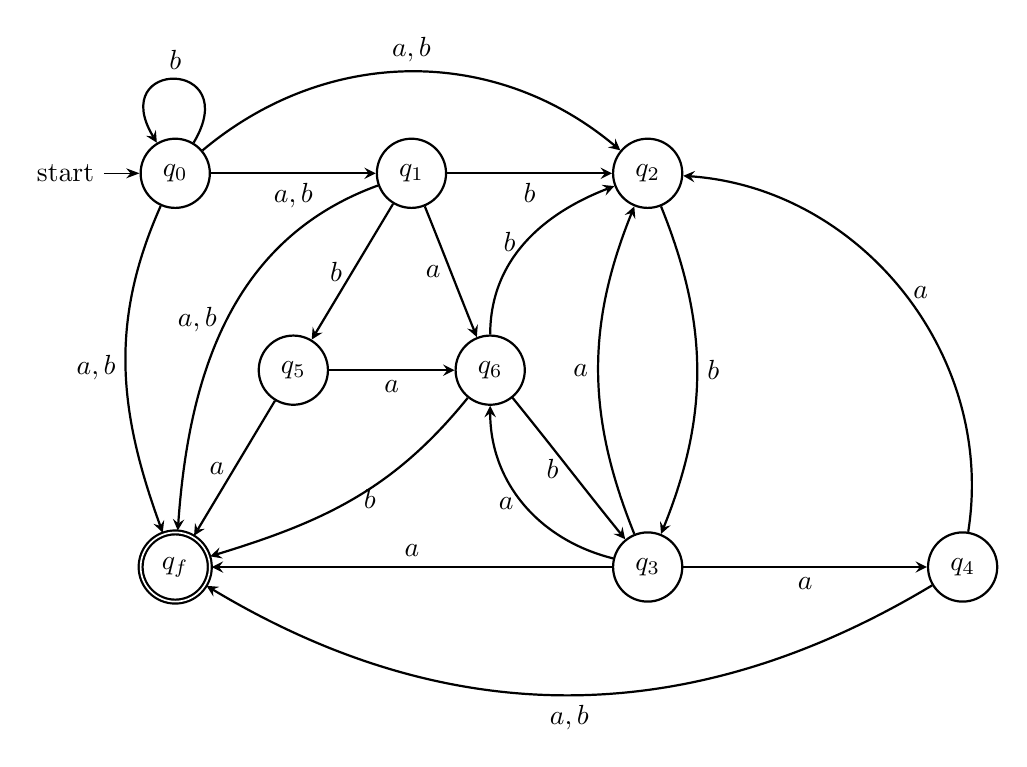
\begin{tikzpicture}[]
    \node[initial,thick,state] at (-7.25,4.5) (32cc4463) {$q_0$};
    \node[thick,state] at (-4.25,4.5) (9914d203) {$q_{1}$};
    \node[thick,state] at (-1.25,4.5) (d5e5a881) {$q_{2}$};
    \node[thick,accepting,state] at (-7.25,-0.5) (64a8b239) {$q_{f}$};
    \node[thick,state] at (-1.25,-0.5) (d4575d37) {$q_{3}$};
    \node[thick,state] at (-5.75,2) (a017ea14) {$q_{5}$};
    \node[thick,state] at (2.75,-0.5) (f0374ef2) {$q_{4}$};
    \node[thick,state] at (-3.25,2) (4a007712) {$q_{6}$};
    \path[->, thick, >=stealth]
    (32cc4463) edge [below,in = 180, out = 0] node {$a,b$} (9914d203)
    (32cc4463) edge [above,in = 140, out = 40] node {$a,b$} (d5e5a881)
    (32cc4463) edge [left,in = 110, out = -114] node {$a,b$} (64a8b239)
    (32cc4463) edge [loop,min distance = 1.25cm,above,in = 121, out = 59] node {$b$} (32cc4463)
    (9914d203) edge [below,in = 180, out = 0] node {$b$} (d5e5a881)
    (9914d203) edge [left,in = 86, out = -160] node {$a,b$} (64a8b239)
    (9914d203) edge [left,in = 59, out = -121] node {$b$} (a017ea14)
    (9914d203) edge [left,in = 112, out = -68] node {$a$} (4a007712)
    (d5e5a881) edge [right,in = 68, out = -68] node {$b$} (d4575d37)
    (d4575d37) edge [above,in = 0, out = 180] node {$a$} (64a8b239)
    (d4575d37) edge [left,in = -112, out = 112] node {$a$} (d5e5a881)
    (d4575d37) edge [below,in = 180, out = 0] node {$a$} (f0374ef2)
    (d4575d37) edge [left,in = -90, out = 166] node {$a$} (4a007712)
    (a017ea14) edge [left,in = 59, out = -121] node {$a$} (64a8b239)
    (a017ea14) edge [below,in = 180, out = 0] node {$a$} (4a007712)
    (f0374ef2) edge [below,in = -31, out = -149] node {$a,b$} (64a8b239)
    (f0374ef2) edge [right,in = -4, out = 81] node {$a$} (d5e5a881)
    (4a007712) edge [right,in = 17, out = -129] node {$b$} (64a8b239)
    (4a007712) edge [left,in = 129, out = -51] node {$b$} (d4575d37)
    (4a007712) edge [left,in = -159, out = 90] node {$b$} (d5e5a881)
    ;
\end{tikzpicture}
\end{center}

The NFA is correct because it accounts for all possible combinations of a and b that do not have the combinations aaa nor abb with zero or more b's trailing. The NFA accounts for when these combinations may occur in a string, as for example abb may occur at an even or odd index within the string. The NFA also accounts for the fact that abb is only an acceptable string if it is followed by an a, as this would invalidate the criteria for abb(b)*. Finally, the NFA also accounts for the fact that there can be at most two a's in a row, and forces the NFA to transition to a b, or accepting state is there are two a's in a row.

\end{document}